\documentclass[a4paper,11pt]{article}
\title{扫码机与图像传感器}
\usepackage{xeCJK}
\usepackage{graphicx}
\usepackage{indentfirst}
\usepackage[colorlinks,linkcolor=blue]{hyperref}

\renewcommand{\figurename}{图}
\usepackage[]{caption2}
\renewcommand{\captionlabeldelim}{}



% \bibliography{citation.bib}

\begin{document}
\setlength{\parindent}{2em}
   \maketitle
   \section{Scanner结构和工作流程}
常见的平板式扫描枪一般由光源、光学透镜、扫描模组、模拟数字转换电路加塑料外壳构成。
	
它利用光电元件将检测 到的光信号转换成电信号,再将电信号通过模拟数字转换器转化为数字信号传输到计算机中处理。当扫描一副图像的时候,光源照射到图像上后反射光穿过透镜会聚到扫描模组上,由扫描模组把光信号转换成模拟数字信号(即电压,它与接受到的光的强度有关),同时指出那个像数的灰暗程度。这时候模拟-数字转换电路把模拟电压转换成数字讯号,传送到电脑。颜色用RGB三色的8、10、12位来量化,既把信号处理成上述位数的图像输出。如果有更高的量化位数,意味着图像能有更丰富的层次和深度,但颜色范围已超出人眼的识别能力,所以在可分辨的范围内对于我们来说,更高位数的扫描枪扫描出来的效果就是颜色衔接平滑,能够看到更多的画面细节。
\\
\\
条码扫描器/模组:
\begin{itemize}
\item[1.] \href{http://www.sumlung.com/cn/2d-barcode-reader.html}{夏浪科技SUMLUNG SL-QC15S 二维码读取器}  
\item[2.] \href{https://www.zebra.com/us/en/products/scanners/general-purpose-scanners/handheld/ds8100-series.html}{DS8100 SERIES CORDED AND CORDLESS 1D/2D HANDHELD IMAGERS——Zebra Tech}
\item[3.] \href{http://www.rakinda.com.cn/cn/productdetail/3/76/41.html}{EM3096二维条码扫描模组}

\end{itemize}

\section{\href{https://www.eefocus.com/embedded/311751/r0}{一款二维条码扫描器系统介绍}}
二维条码扫描器系统框图如图\ref{fig:sys}所示。CMOS图像传感芯片为光电转换元件,用与采集二维条码图像,直接输出为数字信号。由外部扩展SRAM存储该数据,再送到DSP,进行图像处理、码字分割、码字识别、信号纠错等,当一组二维条码信息的识别完成以后,服务程序控制I/O接口给出中断申请信号,DSP响应此中断申请,进入中断服务程序。译码后的二维条码数据从I/O口经SCI RS-232传送至计算机,并在屏幕上显示。软件程序和PDF417码本都储存在DSP芯片中的FLASH内,而动态采集到的二维条码图象数据则储存在SRAM内。
	\begin{figure}
               \begin{center}
               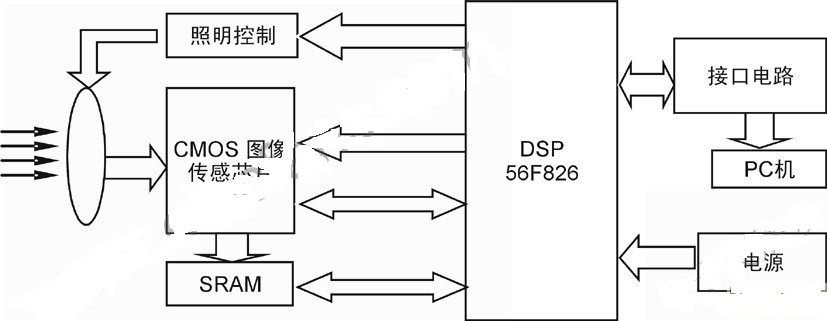
\includegraphics[scale=0.5]{sys.jpg}
               \caption{系统框图}
               \label{fig:sys}
               \end{center}
         \end{figure}
\\
        
系统硬件电路主要包括以下七个部分:条码图象采集电路、DSP主控电路、存储器扩展电路、输出接口电路、复位与时钟电路、电源控制电路、照明控制电路。

其中,条码图象采集电路以OV7120黑白图像传感芯片为核心,该芯片分辨率达到640×480像素,成像速度为30帧/秒,采取逐行扫描方式,输出为数字信号。此芯片功耗低,价格便宜,虽然CCD芯片在信噪比、灵敏度、成像质量等方面优于CMOS芯片,但在本系统设计中,采用CMOS芯片较为合适。

条码图像采集电路图\ref{fig:part1}中,Y0-Y7为总线数字输出,HREF为水平参考信号,即行扫描信号;VSYN为垂直同步信号,即场同步信号。PCLK为像素时钟输出。该电路使用5V直流电,由电源控制电路提供。虽然该芯片使用5V工作电压,但它提供3.3V的I/O口,所以它可以与I/O电压为3.3V的DSP直接相连接,不需要电平转换。当DSP接收到VSYN信号时,表示芯片开始采集第一帧条码图像数据,随后接收到HREF信号,芯片开始进行第一行的数据采集,每来一个PCLK信号,芯片就采集一个像素点的信号,当DSP接收到下一个HREF信号,芯片就进行第二行的数据采集,直到采集完640行的数据,芯片停止采集。当DSP收到下一个VSYN信号时,表示芯片采集下一帧的数据。
	\begin{figure}
               \begin{center}
               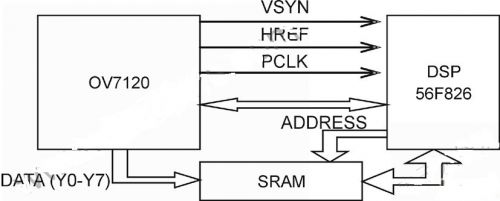
\includegraphics[scale=0.5]{part1.jpg}
               \caption{条码图像采集电路框图}
               \label{fig:part1}
               \end{center}
         \end{figure}

\section{图像传感器}
\subsection{CMOS图像传感器(CIS)}
CMOS图像传感器是一种典型的固体成像传感器。CMOS图像传感器通常由像敏单元阵列、行驱动器、列驱动器、时序控制逻辑、AD转换器、数据总线输出接口、控制接口等几部分组成,这几部分通常都被集成在同一块硅片上。其工作过程一般可分为复位、光电转换、积分、读出几部分。

在CMOS图像传感器芯片上还可以集成其他数字信号处理电路,如AD转换器、自动曝光量控制、非均匀补偿、白平衡处理、黑电平控制、伽玛校正等,为了进行快速计算甚至可以将具有可编程功能的DSP器件与CMOS器件集成在一起,从而组成单片数字相机及图像处理系统。

噪声的大小直接影响CMOS图像传感器对信号的采集和处理,因此如何提高信噪比是CMOS图像传感器的关键技术之一。噪声主要包括散粒噪声、热噪声、1/f噪声、非均匀噪声和固定图像噪声。其中散粒噪声和热噪声是由载流子引起的,1/f噪声和非均匀噪声是由材料的缺陷和不均匀性引起的,固定图像噪声是因为工艺的误差使相邻输出信号的源跟随器不匹配引起的。
 知名图像传感器生产商主要有Sony,Samsung,OmniVision Technologies,ON Semiconductor,Canon等。\\
 \href{https://zhuanlan.zhihu.com/p/27463125}{知乎链接:CMOS图像传感器的过去、现在和未来}  
 \subsection{CCD}
电荷耦合器件(CCD)是20世纪70年代初发展起来的一种新型半导体器件。CCD广泛应用在数码摄影、天文学,尤其是光学遥测技术、光学与频谱望远镜和高速摄影技术,如Lucky imaging。

CCD图像传感器可直接将光学信号转换为模拟电流信号,电流信号经过放大和模数转换,实现图像的获取、存储、传输、处理和复现。其显著特点是:
\begin{itemize}
\item[1.] 体积小重量轻;
\item[2.] 功耗小,工作电压低,抗冲击与震动,性能稳定,寿命长;
\item[3.] 灵敏度高,噪声低,动态范围大;
\item [4.]响应速度快,有自扫描功能,图像畸变小,无残像;
\item [5.]应用超大规模集成电路工艺技术生产,像素集成度高,尺寸精确,商品化生产成本低。因此,许多采用光学方法测量外径的仪器,把CCD器件作为光电接收器。
\end{itemize}

CCD从功能上可分为线阵CCD和面阵CCD两大类。线阵CCD通常将CCD内部电极分成数组,每组称为一相,并施加同样的时钟脉冲。所需相数由CCD芯片内部结构决定,结构相异的CCD可满足不同场合的使用要求。线阵CCD有单沟道和双沟道之分,其光敏区是MOS电容或光敏二极管结构,生产工艺相对较简单。它由光敏区阵列与移位寄存器扫描电路组成,特点是处理信息速度快,外围电路简单,易实现实时控制,但获取信息量小,不能处理复杂的图像。面阵CCD的结构要复杂得多,它由很多光敏区排列成一个方阵,并以一定的形式连接成一个器件,获取信息量大,能处理复杂的图像。

%\begin{refsection}
\section{相机指纹}
由于制造工艺的限制,每一个成像传感器都存在与其他传感器不同的内在缺陷,这种缺陷会以噪声的形式反映在图像上。成像传感器输出的噪声除了量化噪声外,主要由两部分组成:散粒噪声(shot noise)和模式噪声(pattern noise)。其中,散粒噪声为随机部分;而模式噪声为固定成分,其组成如图\ref{fig:noise}所示,其中的Low-frequency defects是由拍照环境引起的影响。
\\

模式噪声的主要由两个部分组成:FPN(fixed pattern noise)和PRNU(photo-response non-uniformity noise)。其中FPN为加性噪声,主要由成像传感器的暗电流产生,会受到温度的影响;PRNU为乘性噪声。这种名为PRNU(photo-response non-uniformity noise)的噪声可以视为成像传感器独一无二的指纹,用于实现数字图像的溯源。因为这种噪声由传感器自身制造缺陷产生,所以也可以将其作为成像传感器强制插入的唯一认证水印。

固定模式噪声(FPN)是由暗电流引起的,它主要指传感器阵列未暴露在光线下时的像素间的差异,主要取决于曝光强度和拍摄温度。由于 FPN 是一种 加性噪声,一些厂商会通过从拍摄的每张图像中减去一个暗场景来自动抑制这种噪 声。

在自然图像中,模式噪声的主要部分是PRNU噪声。而PRNU噪声的主要成因是pixel non-uniformity (PNU)即各个像素对光的敏感度不同,这是由硅片的不均匀性和传感器制造过程中的缺陷引起的,因此PNU噪声是传感器的固有特性,且不受拍摄温度和湿度的影响。

以上内容摘自参考文献

《\href{https://www.researchgate.net/publication/3455253_Digital_Camera_Identification_From_Sensor_Pattern_Noise?enrichId=rgreq-d1a8e8e6a055ab936531c60ca2752109-XXX&enrichSource=Y292ZXJQYWdlOzM0NTUyNTM7QVM6MjMxNTYwMjQyNzkwNDAwQDE0MzIyMTk2NzIyMjg\%3D&el=1_x_3&_esc=publicationCoverPdf}{Digital Camera Identification From Sensor Pattern Noise}》 P2-P3
\begin{figure}[!htbp]
	\centering
	%\begin{center}
	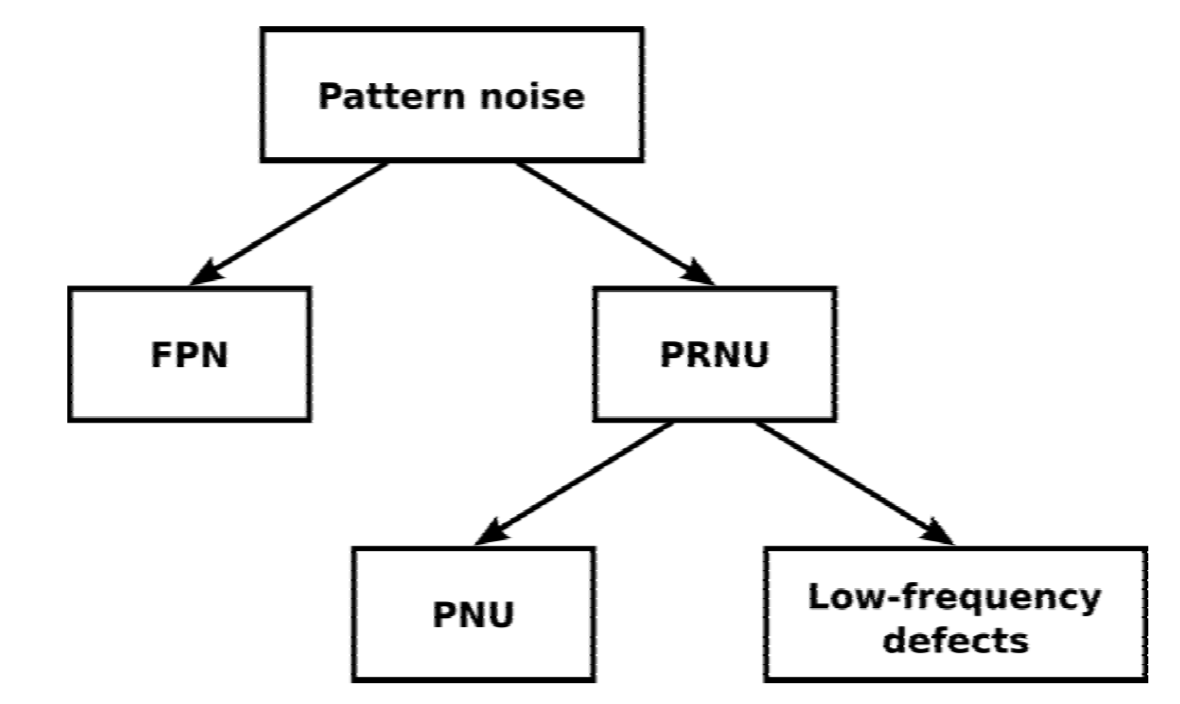
\includegraphics[scale=0.3]{noise.png}
	\caption{Pattern noise of image sensors.}
	\label{fig:noise}
	%\end{center}
\end{figure}


\end{document}